% SOICT 2026 submission - Springer LNCS format (single-blind: keep author names).
% Requires the Springer LNCS class `llncs.cls` + `splncs04.bst`.
% Multi-market volatility forecasting model. Figures in docs/paper/figures/.
% MODEL SWAP 2026-09-18: GBM/GBME (HGBR) rows replaced by XGBoost gamma variants (capacity-matched).
%   XGB (earn) + XGB+leafgraph, all horizons 8 folds: results/gamma_gbm/leaf_graph_hose_h{1,5,10,22}.json
%     (keys GBME/XGB/XGB+leafgraph + dm + gain_pct + spike_robustness + alpha) and leaf_graph_sp500_h{1,5,10,22}.json.
%   XGB (no-earn) HOSE: results/gamma_gbm/leaf_graph_paper_hose_noearn_h{1,5,10,22}.json (8 folds).
%   XGB (no-earn) SP500: results/gamma_gbm/leaf_graph_paper_sp500_noearn_h{1,5,10,22}.json (8 folds).
%   GARCH MSE/RMSE/MAE added 2026-09-18 (garch_<market>.json metrics; scored over GARCH estimable subset).
% Benchmark rows UNCHANGED: HAR = full_compare_<market>.json + paper_metrics_<market>.json;
%   GNNHAR = gnnhar_<market>.json; GARCH = garch_<market>.json.
\documentclass{llncs}
\usepackage{graphicx}
\graphicspath{{figures/}}
\usepackage{booktabs}
\usepackage{amsmath}
\usepackage{amssymb}
\usepackage{placeins}
\usepackage[utf8]{inputenc}
\usepackage[T1,T5]{fontenc}

\begin{document}

\title{Multi-Market Stock Volatility Forecasting Model}

\author{Thanh-Quy Nguyen \and Trung-Hoang Le \and Duy-Hoang Tran}
\institute{University of Science, Vietnam National University Ho Chi Minh City, Ho Chi Minh City, Vietnam \\ \email{lthoang@hcmus.edu.vn}}

\maketitle

\begin{abstract}
Forecasting daily stock-price volatility, how much a stock's price is likely to swing on a given day,
is a core input to risk management and option pricing: a risk manager sizing exposure or a trader
pricing an option needs to know not only which direction a price may move but how large its swings
will be. We build a per-stock volatility forecasting model on a gamma-loss gradient-boosted tree
ensemble (XGBoost) over endogenous (own-history) features, and we ask where extra information actually helps. The
endogenous model beats the HAR linear benchmark, a per-stock GARCH, and a learned graph
neural network (GNNHAR) on QLIKE at every horizon. We then study two external levers on two
structurally different markets. On the S\&P~500, adding a forward-looking scheduled-earnings feature
is the dominant lever, cutting QLIKE by 14 to 16\% over the HAR baseline at every horizon
(Diebold-Mariano $p<0.001$); on 405 Vietnam Ho Chi Minh Stock Exchange (HOSE) tickers the earnings
lever does not transfer, which localizes the earnings gain to the S\&P~500. Conversely, a
leaf-cooccurrence graph that smooths each trading day's cross-section of forecasts, built from the
boosted model's own tree leaves with a smoothing weight fit on validation data, lowers HOSE QLIKE at
the one-, five-, and ten-day horizons by 0.12 to 0.26\% (Diebold-Mariano $p<0.005$, robust to regime
spikes), whereas on the liquid S\&P~500 the validation-fit weight collapses toward zero and the graph
is inert. The graph is therefore a thin-market cross-sectional denoising effect rather than a
universal one.
\keywords{Volatility forecasting \and HAR \and Gradient boosting \and Earnings announcements \and Graph smoothing \and Diebold-Mariano.}
\end{abstract}

\section{Introduction}
Financial markets are volatile: prices swing, and the size of those swings, an asset's
\emph{volatility}, is the standard measure of its risk. Because volatility drives how options are
priced, how much capital a position ties up, and how risk is budgeted across a portfolio, forecasting
it accurately is a long-standing problem in financial econometrics~\cite{corsi2009}. Volatility is
not observed directly; it is estimated from prices, so any forecast is a forecast of an estimate. We
target the daily \emph{Parkinson estimator}~\cite{parkinson1980}, which gauges a day's variance from
its high-low price range and uses more of the day's information than a close-to-close measure; our
forecasting target is therefore a variance (a squared quantity), not a standard deviation.

The standard linear approach is the HAR family~\cite{corsi2009}: a plain linear regression that
predicts tomorrow's volatility from its own averages over the last day, the last week (about five
trading days), and the last month (about twenty-two), summarising volatility's long memory with a
handful of coefficients. This benchmark is deliberately simple yet hard to beat. We build a stronger
per-stock gradient-boosted tree model (a gamma-loss XGBoost ensemble) on top of it and ask what extra
information actually helps. As a learned-model reference we also train a graph neural network on the
HAR features~\cite{gnnhar2024} and measure it under the same protocol.

We forecast daily Parkinson variance with a per-stock gamma-loss XGBoost model over endogenous
features, then study two external levers under a leakage-controlled walk-forward protocol scored on
QLIKE with date-clustered Diebold-Mariano tests. The first lever is forward-looking and specific to
the firm: a scheduled earnings release is known weeks ahead and raises volatility around the
announcement~\cite{patell1981}, and encoding the distance from the forecast target to the nearest
scheduled release is the dominant lever on the S\&P~500. The second lever is cross-sectional: on the
thin HOSE market a graph that connects stocks whose forecasts follow similar paths through the boosted
model's trees, and averages their same-day forecasts, denoises the prediction and lowers QLIKE, while
on the liquid S\&P~500 that graph self-disables. A learned graph neural network (GNNHAR), by contrast,
does not beat the endogenous model on either market.

This paper contributes three results. First, a per-stock gamma-loss XGBoost model over endogenous
features is a strong, transparent baseline for daily volatility that beats HAR, a per-stock
GARCH, and a learned graph neural network (GNNHAR) at every horizon. Second, a forward-looking
scheduled-earnings feature is the dominant external lever on the S\&P~500, cutting QLIKE by 14 to
16\% over the HAR baseline at every horizon (Diebold-Mariano $p<0.001$); we replicate the study on a
second market, 405 Vietnam HOSE tickers, where the earnings lever does not transfer, which localizes
the earnings gain to the S\&P~500. Third, a leaf-cooccurrence graph that denoises each trading day's
cross-section of forecasts lowers HOSE QLIKE at the one-, five-, and ten-day horizons
(Diebold-Mariano-significant and robust to regime spikes) yet self-disables on the liquid S\&P~500,
identifying it as a thin-market cross-sectional denoising phenomenon rather than a universal one.

\paragraph{Terminology.}
\emph{Volatility}: the size of a stock's price fluctuations, the standard proxy for its risk.
\emph{Parkinson estimator}: a day's variance measured from its high-low price range; our forecasting
target is this variance (squared units), not the standard deviation.
\emph{HAR}: a linear model predicting volatility from its own daily, weekly, and monthly averages.
\emph{QLIKE}: a proxy-robust error measure for volatility forecasts that stays reliable when the
target is a noisy proxy~\cite{patton2011}.
\emph{Diebold-Mariano (DM) test}: a test of whether one forecast is more accurate than another by
more than chance, computed from their day-by-day loss differences~\cite{dm1995}.
\emph{Horizon} $h$: how many trading days ahead we forecast ($h\in\{1,5,10,22\}$, roughly a day, week,
fortnight, and month).

\section{Method and Setup}
\textbf{Target and metric.} We forecast daily Parkinson variance
$\mathrm{pk}_t=\ln(H_t/L_t)^2/(4\ln 2)$ from the daily high $H$ and low $L$, at horizons $h\in\{1,5,10,22\}$ over 497 S\&P~500 constituents. We report QLIKE as the
primary loss~\cite{patton2011}, alongside MSE, RMSE and MAE. We test significance with a
Diebold-Mariano statistic~\cite{dm1995} on per-trading-date mean loss, with the
Harvey-Leybourne-Newbold small-sample correction~\cite{hln1997}, because within-day stock errors are
dependent.

\textbf{Data sources.} Daily OHLCV for the 497 S\&P~500 constituents is obtained from Yahoo Finance
(via the \texttt{yfinance} library); the 405 HOSE constituents are obtained from \texttt{vnstock}, a
Vietnamese market-data feed, with each ticker's full daily history crawled from its exchange listing. The
Parkinson variance target and all endogenous own-history features are derived from the daily high, low,
and close prices. The earnings dates and their provenance (Yahoo Finance for the S\&P~500; the State
Securities Commission disclosure portal together with a \texttt{vnstock} news feed for HOSE) are described
in the Limitations.

\textbf{Model.} The forecasting model is a per-stock gamma-loss gradient-boosted tree
ensemble~\cite{friedman2001} (XGBoost~\cite{chen2016} with the \texttt{reg:gamma} objective, whose
deviance equals QLIKE up to a constant: 300 boosting rounds, learning rate 0.05, at most 31 leaves per
tree under a loss-guided grow policy, L2 penalty 1.0, minimum child weight 20, 3-seed ensemble). The endogenous feature vector is $\mathbb{R}^8$: three HAR
lags~\cite{corsi2009} and five log-volatility momentum terms. An External earnings block
(denoted \textbf{XGB+E}) extends it: $\mathbb{R}^4$ of forward-looking scheduled-earnings features,
chiefly the distance from the forecast target to the nearest scheduled release. A leaf-cooccurrence
graph (denoted \textbf{XGB+E+LG}) smooths the resulting forecasts across each day's
cross-section. Figure~\ref{fig:arch} shows the architecture.

\textbf{Baselines.} HAR~\cite{corsi2009} fits three endogenous lags by ordinary least squares. GARCH is a per-stock GARCH(1,1) on daily
returns. GNNHAR~\cite{gnnhar2024} is a learned graph neural network (two graph-convolution layers over
the three HAR lags, its best variant). All share the same target, protocol, and positivity floor as
the XGBoost model.

\subsection*{Features}
\textbf{Endogenous block (8 features, used by XGB).} Every endogenous feature is observable at the
forecast origin $t$. The three HAR lags capture short, medium, and long memory of realized variance
over one day, one trading week ($\mathrm{WK}=5$), and one trading month (22 days):
\begin{align}
\mathrm{har\_daily} = \mathrm{pk}_t, \qquad
\mathrm{har\_weekly} = \frac{1}{5}\sum_{k=0}^{4}\mathrm{pk}_{t-k}, \qquad
\mathrm{har\_monthly} = \frac{1}{22}\sum_{k=0}^{21}\mathrm{pk}_{t-k}.
\end{align}
Five log-volatility momentum terms, built on $\ell_t=\ln(\max(\mathrm{pk}_t,\varepsilon))$ with
$\varepsilon=10^{-8}$, encode recent trend, multi-scale slope, deviation from the recent mean, and a
standardized 22-day level:
\begin{align}
\mathrm{mr\_change} &= \ell_t-\ell_{t-1}, &
\mathrm{mr\_slope5} &= \frac{\ell_t-\ell_{t-5}}{5}, &
\mathrm{mr\_slope10} &= \frac{\ell_t-\ell_{t-10}}{10},\\
\mathrm{mr\_dev5} &= \ell_t-\frac{1}{5}\sum_{k=0}^{4}\ell_{t-k}, &
\mathrm{mr\_z22} &= \frac{\ell_t-\mu_{22}(\ell)}{\sigma_{22}(\ell)+\varepsilon}, &&
\end{align}
where $\mu_{22}$ and $\sigma_{22}$ are the trailing 22-day mean and standard deviation of $\ell$.
Together these summarize the stock's own short-run acceleration and regime level.

\textbf{External earnings block (4 features, used by XGB+E).} Each earnings feature is evaluated at the
target day $t+h$ from scheduled release dates known weeks ahead, so the block is forward-looking,
though built from realized announcement dates rather than a point-in-time scheduling snapshot (a caveat
quantified in the Limitations). Let $\mathrm{nxt}$ be the trading days from $t+h$ to the next scheduled announcement,
$\mathrm{prv}$ the trading days since the previous one, and $\mathrm{dist}=\min(\mathrm{nxt},\mathrm{prv})$:
\begin{align}
\mathrm{earn\_prox} &= \max\!\Big(0,\,1-\tfrac{\mathrm{dist}}{5}\Big), &
\mathrm{earn\_soon} &= \mathbf{1}[\mathrm{dist}\le 3],\\
\mathrm{earn\_pre} &= \max\!\Big(0,\,1-\tfrac{\mathrm{nxt}}{5}\Big), &
\mathrm{earn\_post} &= \max\!\Big(0,\,1-\tfrac{\mathrm{prv}}{10}\Big).
\end{align}
Here $\mathrm{earn\_prox}$ is a symmetric triangular proximity that peaks at 1 on the announcement day
and reaches 0 once the nearest release is at least a week away, $\mathrm{earn\_soon}$ is a sharp
$\pm 3$-day flag, $\mathrm{earn\_pre}$ rises into the next release, and $\mathrm{earn\_post}$ decays
over a longer 10-day window because post-earnings volatility drift persists longer than the
pre-announcement run-up. Away from any release all four are zero, so XGB+E reduces to XGB on ordinary
days and activates only in the roughly two-week window around a scheduled release.
Figure~\ref{fig:eventstudy} shows the S\&P~500 median variance rises to about 2.75 times baseline on
the announcement day, which motivates these windows; on HOSE the median stays flat, so the block is
inert there.

\begin{figure}[t]
\centering
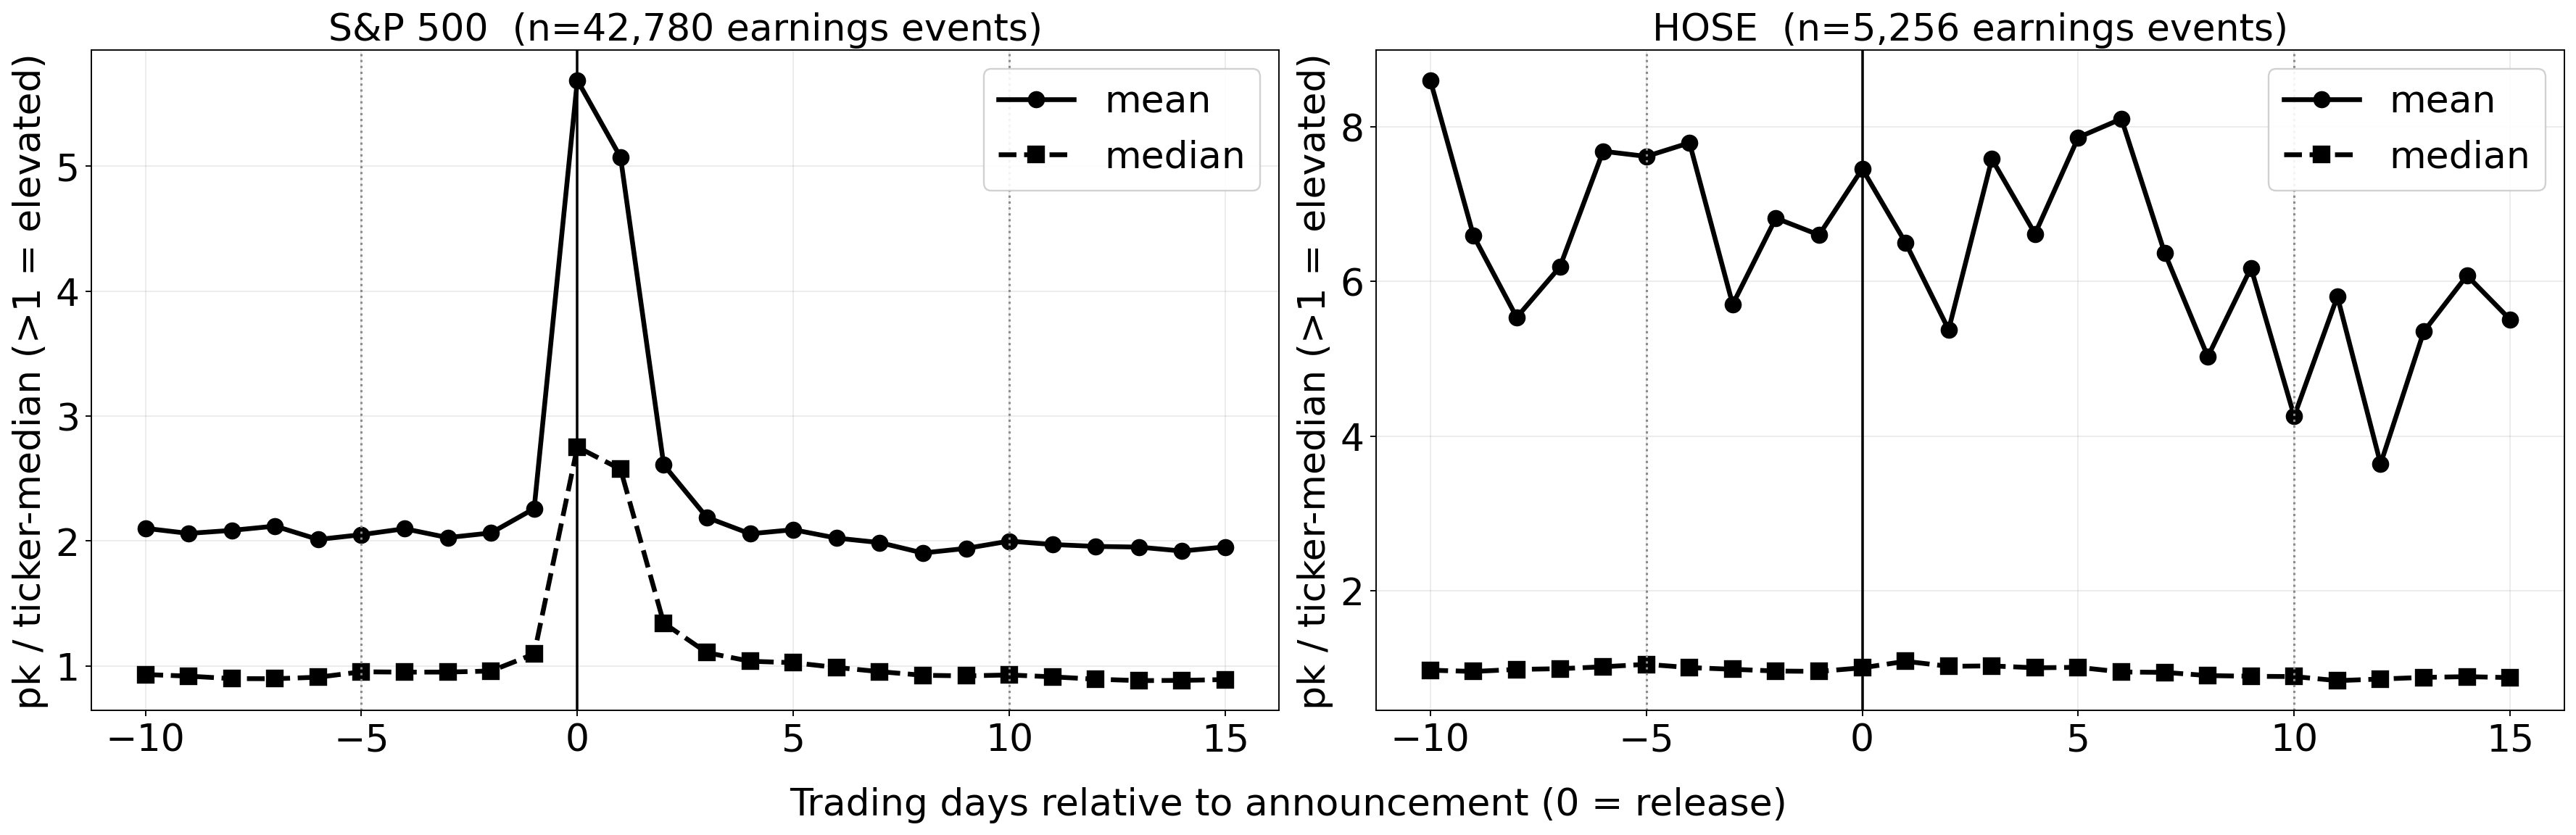
\includegraphics[width=\linewidth]{figures/fig_earnings_event_study.png}
\caption{Event study: median realized Parkinson variance (normalised by each ticker's median) versus
trading days from a scheduled earnings release. The S\&P~500 median rises to about 2.75 times baseline
on the announcement day and returns within roughly a week; the HOSE median stays near one at every
offset, showing no announcement spike, which is why the earnings feature helps the S\&P~500 but not
HOSE.}
\label{fig:eventstudy}
\end{figure}

\textbf{Protocol.} We use expanding-window walk-forward folds with a target-horizon gap. All
correlations, adjacencies, factor estimates, and model fits use training data only; the test window is
read once. Every gradient-boosting model averages three seeds. Predictions are floored identically
across models before scoring.

\textbf{Leaf-cooccurrence graph (XGB+E+LG).} The graph reuses the fitted booster to denoise its own
forecasts across the same-day cross-section, adding no information beyond the trees. For each stock on
each test day we read the vector of leaf indices the 300 trees assign to it; two stocks are similar
when many trees route them to the same leaf, so the fraction of shared leaves is a Hamming similarity
in $[0,1]$~\cite{chen2016}. This construction is the boosted-tree analogue of the random-forest
proximity (leaf-incidence) kernel~\cite{rhodes2023}. Within each trading day we build a $k$-nearest-neighbour
graph ($k=10$) over that similarity and replace each stock's forecast by
$\hat y_i^{\,\mathrm{LG}}=(1-\alpha)\,\hat y_i+\alpha\,\overline{\hat y}_{\mathcal{N}(i)}$, where
$\overline{\hat y}_{\mathcal{N}(i)}$ is the mean forecast over its neighbours. The smoothing weight
$\alpha\in[0,1]$ is selected per fold on the validation slice only and applied once to the test
window, so the graph is causal and can switch itself off ($\alpha=0$) when smoothing does not help in
validation. The graph is built only over the same day's stocks, so it introduces no temporal leakage.

\begin{figure}[t]
\centering
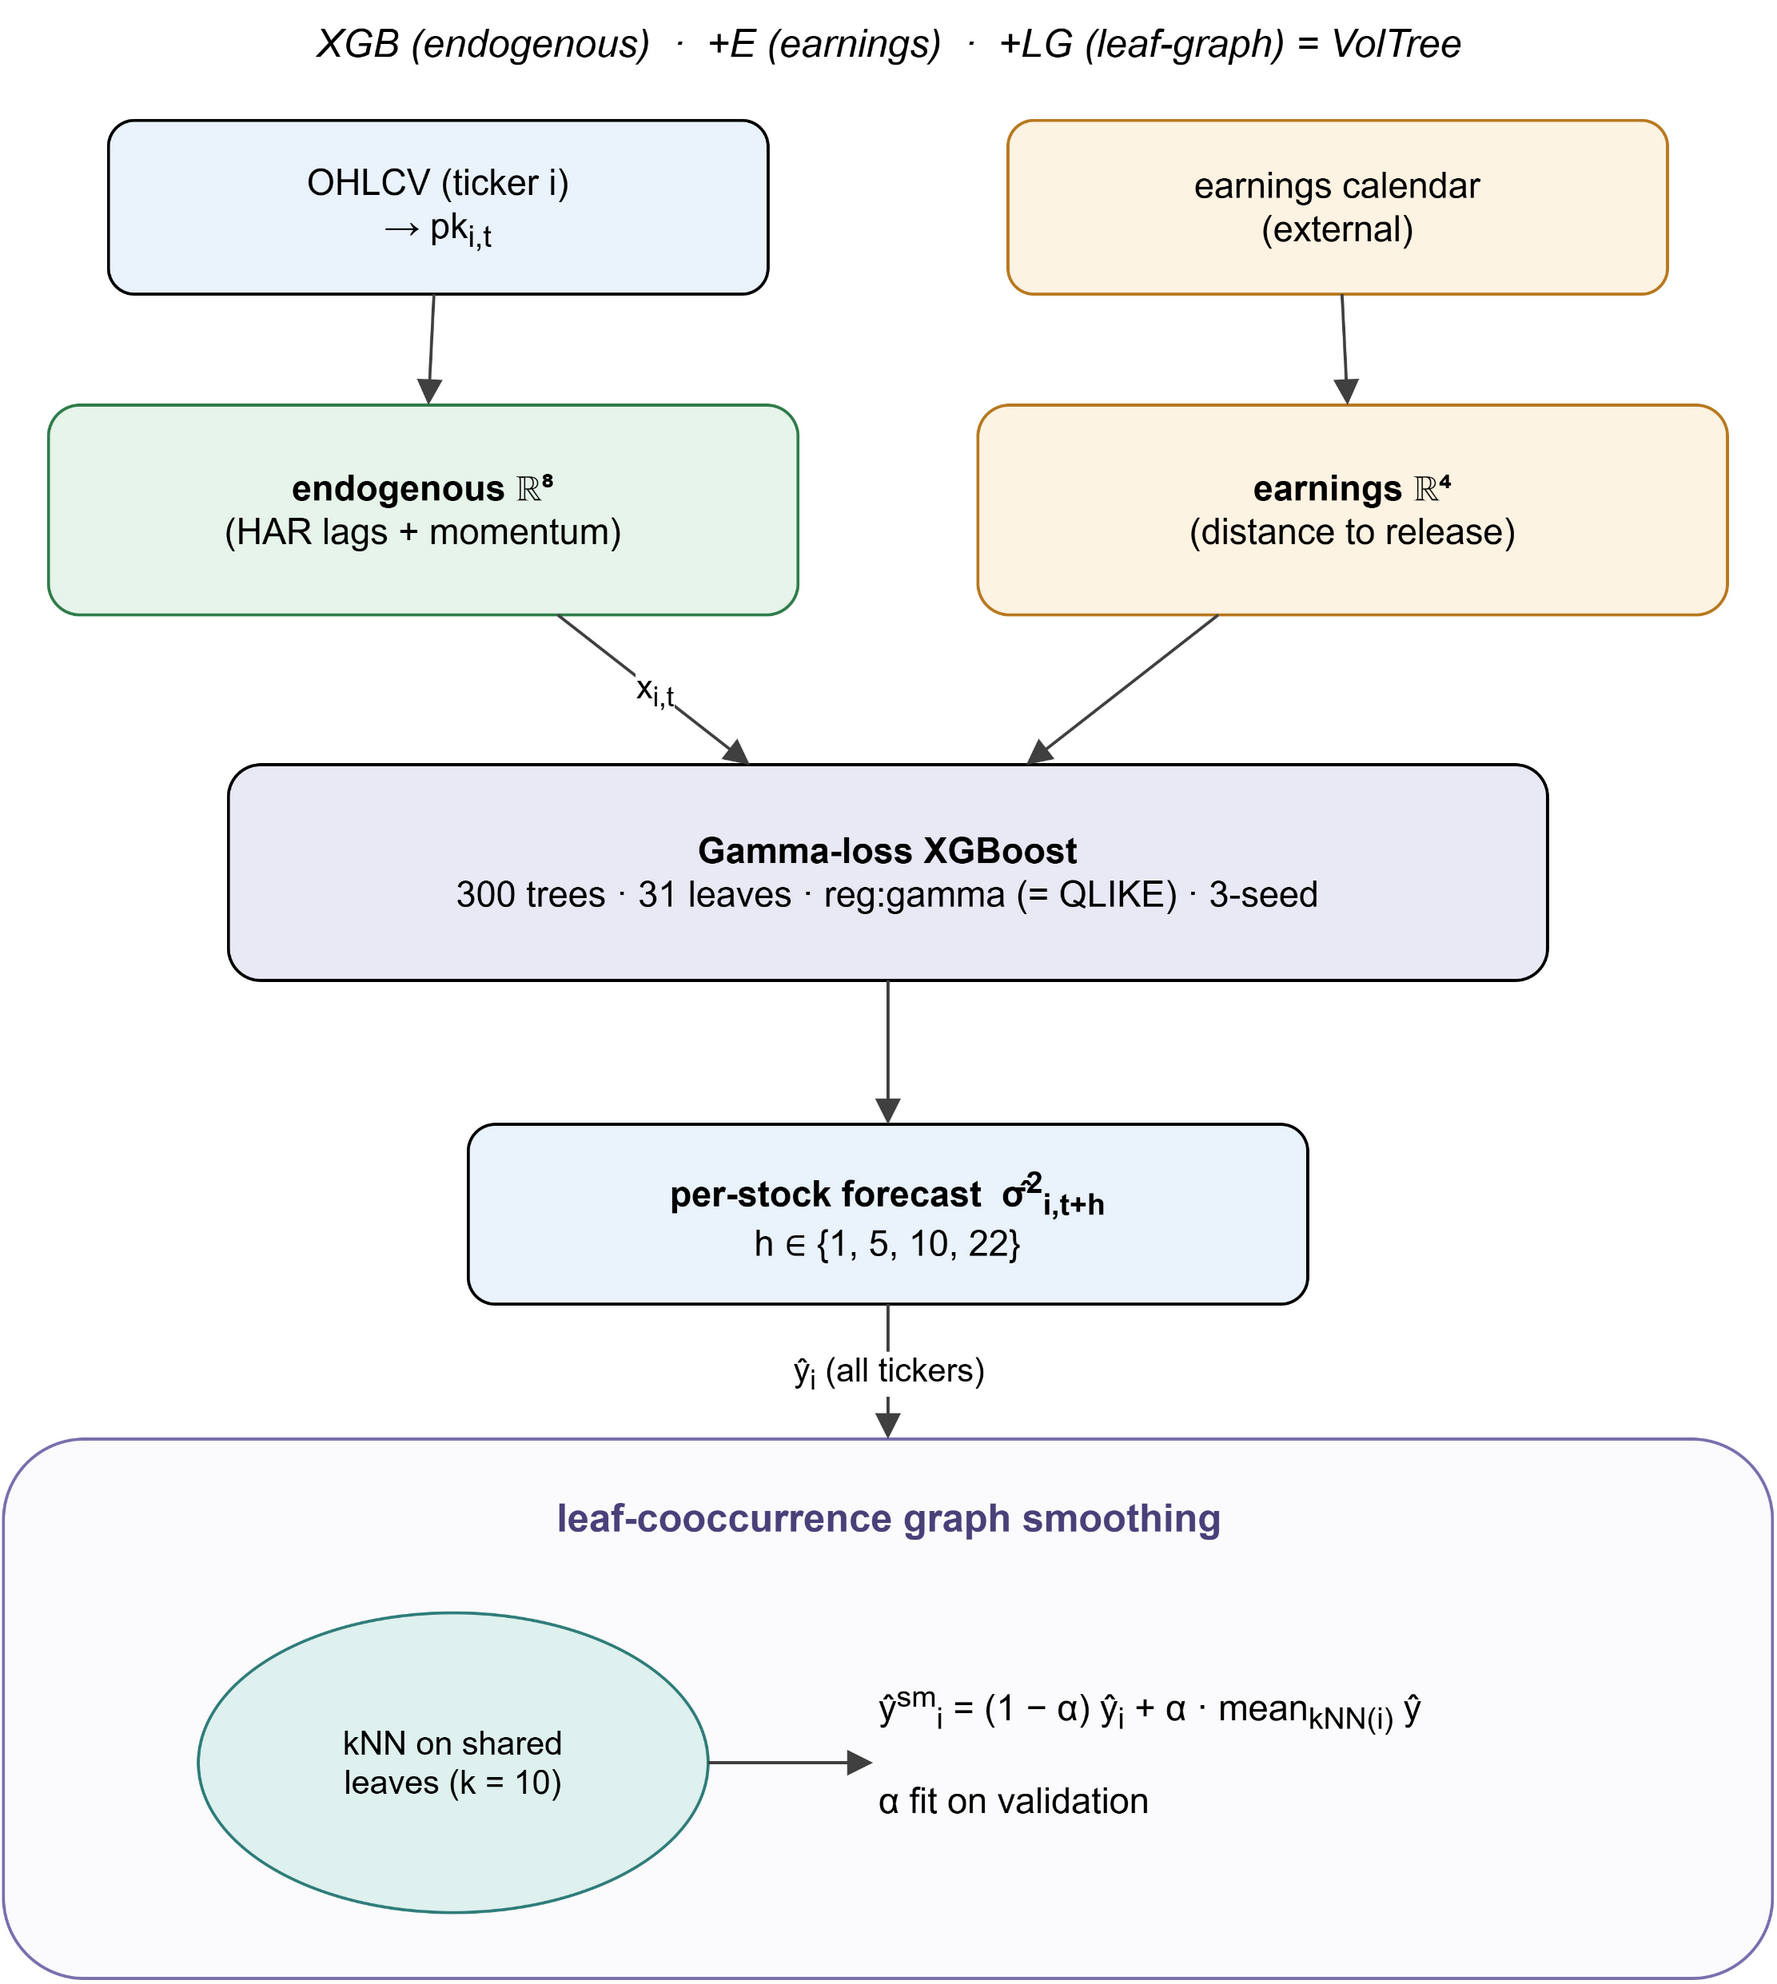
\includegraphics[width=\textwidth]{fig_architecture.png}
\caption{Model architecture. A per-stock feature vector combines endogenous features
($\mathbb{R}^8$: three HAR lags and five log-volatility momentum terms) with an External
forward-looking scheduled-earnings block ($\mathbb{R}^4$). A gamma-loss gradient-boosted tree ensemble
(XGBoost) maps the feature vector to the multi-horizon Parkinson-variance forecast, which a
per-day leaf-cooccurrence graph smooths across the cross-section.}
\label{fig:arch}
\end{figure}

\section{Results: The Endogenous Model Beats the Baselines}\label{sec:graph}
Table~\ref{tab:summary} summarises the headline metrics (MSE, RMSE, MAE, QLIKE) across both markets: the final model XGB+E+LG posts the best value on every metric at every horizon in both, ahead of all three baselines. Table~\ref{tab:sp500} reports all four metrics for the S\&P~500 across GARCH, HAR, the learned
GNNHAR, and the XGBoost variants at every horizon: XGB (endogenous only), XGB+E (endogenous plus the
earnings block), and XGB+E+LG (XGB+E with leaf-graph smoothing). The XGBoost model beats HAR
and GARCH on QLIKE at every horizon, and the learned GNNHAR does not beat it: GNNHAR is worse than the
XGBoost model at every horizon and worse than even linear HAR at the shortest horizon (QLIKE 0.375
against HAR's 0.370 at $h1$), so a multi-hop graph network recovers nothing the endogenous model does
not already capture. The earnings model XGB+E carries the bolded QLIKE in every block; the leaf-graph
smoothing that helps HOSE is inert here, as Section~\ref{sec:hose} explains. The next section isolates
why earnings are the lever.

\begin{table}[t]
\centering
\caption{Headline comparison across both markets: three baselines (GARCH, HAR, GNNHAR) against the paper's
final model XGB+E+LG (endogenous XGBoost with the earnings block and leaf-graph smoothing). All four
metrics (MSE, RMSE, MAE, QLIKE; lower is better) at horizons $h\in\{1,5,10,22\}$; S\&P~500 on the left,
HOSE on the right. MSE $\times10^{-6}$, RMSE/MAE $\times10^{-3}$; QLIKE unscaled (same scaling as
Tables~\ref{tab:sp500} and~\ref{tab:hose}). The final model attains the best value on every metric at every
horizon in both markets. Bold marks the full-precision column minimum among these four models. Per-model
detail with the intermediate XGB and XGB+E variants is in Tables~\ref{tab:sp500} and~\ref{tab:hose}.}
\label{tab:summary}
\footnotesize
\setlength{\tabcolsep}{4pt}
\begin{tabular}{ll cccc cccc}
\toprule
& & \multicolumn{4}{c}{\textbf{S\&P~500}} & \multicolumn{4}{c}{\textbf{HOSE}} \\
\cmidrule(lr){3-6}\cmidrule(lr){7-10}
$h$ & Model & MSE & RMSE & MAE & QLIKE & MSE & RMSE & MAE & QLIKE \\
\midrule
1 & GARCH    & 0.796 & 0.892 & 0.327 & 0.465 & 0.630 & 0.794 & 0.487 & 1.656 \\
1 & HAR      & 0.575 & 0.759 & 0.213 & 0.370 & 0.660 & 0.813 & 0.519 & 1.812 \\
1 & GNNHAR   & 0.576 & 0.759 & 0.212 & 0.375 & 0.585 & 0.765 & 0.438 & 1.682 \\
1 & XGB+E+LG & \textbf{0.541} & \textbf{0.735} & \textbf{0.202} & \textbf{0.317} & \textbf{0.534} & \textbf{0.731} & \textbf{0.391} & \textbf{1.565} \\
\midrule
5 & GARCH    & 0.789 & 0.888 & 0.343 & 0.508 & 0.703 & 0.838 & 0.537 & 1.740 \\
5 & HAR      & 0.614 & 0.784 & 0.230 & 0.436 & 0.663 & 0.814 & 0.523 & 1.822 \\
5 & GNNHAR   & 0.638 & 0.799 & 0.233 & 0.446 & 0.616 & 0.785 & 0.469 & 1.744 \\
5 & XGB+E+LG & \textbf{0.599} & \textbf{0.774} & \textbf{0.218} & \textbf{0.371} & \textbf{0.578} & \textbf{0.760} & \textbf{0.424} & \textbf{1.647} \\
\midrule
10 & GARCH    & 0.757 & 0.870 & 0.349 & 0.522 & 0.734 & 0.857 & 0.565 & 1.782 \\
10 & HAR      & 0.621 & 0.788 & 0.236 & 0.461 & 0.666 & 0.816 & 0.525 & 1.828 \\
10 & GNNHAR   & 0.660 & 0.812 & 0.243 & 0.477 & 0.628 & 0.792 & 0.483 & 1.767 \\
10 & XGB+E+LG & \textbf{0.617} & \textbf{0.786} & \textbf{0.225} & \textbf{0.392} & \textbf{0.595} & \textbf{0.771} & \textbf{0.439} & \textbf{1.682} \\
\midrule
22 & GARCH    & 0.739 & 0.860 & 0.363 & 0.544 & 0.788 & 0.888 & 0.606 & 1.837 \\
22 & HAR      & 0.633 & 0.795 & 0.242 & 0.485 & 0.672 & 0.820 & 0.528 & 1.835 \\
22 & GNNHAR   & 0.635 & 0.797 & 0.241 & 0.476 & 0.655 & 0.809 & 0.507 & 1.810 \\
22 & XGB+E+LG & \textbf{0.609} & \textbf{0.780} & \textbf{0.228} & \textbf{0.407} & \textbf{0.621} & \textbf{0.788} & \textbf{0.460} & \textbf{1.726} \\
\bottomrule
\end{tabular}
\end{table}

\begin{table}[t]
\centering
\caption{Main result, S\&P~500 (497 constituents; walk-forward, 3-seed ensembles). Lower is better
on every metric. MSE $\times10^{-6}$, RMSE/MAE $\times10^{-3}$; QLIKE unscaled. GARCH is a per-stock
GARCH(1,1) benchmark; all its metrics (including the squared-error columns) are scored over its estimable
subset ($\sim$99.5\% of rows), a slightly different sample than the other models. XGB is the
endogenous model, XGB+E adds the earnings block, and XGB+E+LG adds leaf-graph smoothing. Bold marks
the best value in each metric column per horizon; the QLIKE bold additionally requires a significant
date-clustered Diebold-Mariano test ($p<0.05$).}
\label{tab:sp500}
\footnotesize
\setlength{\tabcolsep}{6pt}
\begin{tabular}{llcccc}
\toprule
$h$ & Model & MSE & RMSE & MAE & QLIKE \\
\midrule
1 & GARCH       & 0.796 & 0.892 & 0.327 & 0.465 \\ % garch_sp500.json h1 GARCH (estimable subset; mse 7.956e-7, rmse 8.920e-4, mae 3.271e-4, qlike 0.4649)
1 & HAR         & 0.575 & 0.759 & 0.213 & 0.370 \\ % full_compare_sp500.json h1 metrics.HAR (mse 5.7541e-7, rmse 7.5856e-4, mae 2.1318e-4, qlike 0.36970)
1 & GNNHAR      & 0.576 & 0.759 & 0.212 & 0.375 \\ % gnnhar_sp500.json metrics.GNNHAR_h1 (mse 5.7598e-7, rmse 7.5893e-4, mae 2.1209e-4, qlike 0.37494)
1 & XGB         & 0.558 & 0.747 & 0.209 & 0.357 \\ % leaf_graph_paper_sp500_noearn_h1.json metrics.XGB (n_folds=8; mse 5.5753e-7, rmse 7.4668e-4, mae 2.0927e-4, qlike 0.35726)
1 & XGB+E       & 0.541 & 0.736 & 0.202 & \textbf{0.317} \\ % leaf_graph_sp500_h1.json metrics.XGB
1 & XGB+E+LG    & \textbf{0.541} & \textbf{0.735} & \textbf{0.202} & 0.317 \\ % leaf_graph_sp500_h1.json metrics.XGB+leafgraph (leaf inert, DM p=0.66)
\midrule
5 & GARCH       & 0.789 & 0.888 & 0.343 & 0.508 \\ % garch_sp500.json h5 GARCH (estimable subset; mse 7.891e-7, rmse 8.883e-4, mae 3.427e-4, qlike 0.5077)
5 & HAR         & 0.614 & 0.784 & 0.230 & 0.436 \\ % full_compare_sp500.json h5 metrics.HAR (mse 6.1406e-7, rmse 7.8362e-4, mae 2.2967e-4, qlike 0.43635)
5 & GNNHAR      & 0.638 & 0.799 & 0.233 & 0.446 \\ % gnnhar_sp500.json metrics.GNNHAR_h5 (mse 6.3789e-7, rmse 7.9868e-4, mae 2.3298e-4, qlike 0.44618)
5 & XGB         & 0.613 & 0.783 & 0.226 & 0.412 \\ % leaf_graph_paper_sp500_noearn_h5.json metrics.XGB (n_folds=8; mse 6.1307e-7, rmse 7.8299e-4, mae 2.2620e-4, qlike 0.41210)
5 & XGB+E       & \textbf{0.599} & \textbf{0.774} & 0.219 & \textbf{0.371} \\ % leaf_graph_sp500_h5.json metrics.XGB
5 & XGB+E+LG    & 0.599 & 0.774 & \textbf{0.218} & 0.371 \\ % leaf_graph_sp500_h5.json metrics.XGB+leafgraph
\midrule
10 & GARCH       & 0.757 & 0.870 & 0.349 & 0.522 \\ % garch_sp500.json h10 GARCH (estimable subset; mse 7.571e-7, rmse 8.701e-4, mae 3.494e-4, qlike 0.5218)
10 & HAR         & 0.621 & 0.788 & 0.236 & 0.461 \\ % full_compare_sp500.json h10 metrics.HAR (mse 6.2137e-7, rmse 7.8827e-4, mae 2.3561e-4, qlike 0.46150)
10 & GNNHAR      & 0.660 & 0.812 & 0.243 & 0.477 \\ % gnnhar_sp500.json metrics.GNNHAR_h10 (mse 6.6005e-7, rmse 8.1244e-4, mae 2.4258e-4, qlike 0.47666)
10 & XGB         & 0.631 & 0.794 & 0.232 & 0.431 \\ % leaf_graph_paper_sp500_noearn_h10.json metrics.XGB (n_folds=8; mse 6.3082e-7, rmse 7.9424e-4, mae 2.3245e-4, qlike 0.43112)
10 & XGB+E       & \textbf{0.616} & \textbf{0.785} & 0.225 & \textbf{0.392} \\ % leaf_graph_sp500_h10.json metrics.XGB
10 & XGB+E+LG    & 0.617 & 0.786 & \textbf{0.225} & 0.392 \\ % leaf_graph_sp500_h10.json metrics.XGB+leafgraph
\midrule
22 & GARCH       & 0.739 & 0.860 & 0.363 & 0.544 \\ % garch_sp500.json h22 GARCH (estimable subset; mse 7.392e-7, rmse 8.598e-4, mae 3.630e-4, qlike 0.5442)
22 & HAR         & 0.633 & 0.795 & 0.242 & 0.485 \\ % full_compare_sp500.json h22 metrics.HAR (mse 6.3273e-7, rmse 7.9544e-4, mae 2.4189e-4, qlike 0.48549)
22 & GNNHAR      & 0.635 & 0.797 & 0.241 & 0.476 \\ % gnnhar_sp500.json metrics.GNNHAR_h22 (mse 6.3530e-7, rmse 7.9706e-4, mae 2.4143e-4, qlike 0.47614)
22 & XGB         & 0.623 & 0.789 & 0.236 & 0.446 \\ % leaf_graph_paper_sp500_noearn_h22.json metrics.XGB (n_folds=8; mse 6.2256e-7, rmse 7.8903e-4, mae 2.3593e-4, qlike 0.44595)
22 & XGB+E       & \textbf{0.609} & \textbf{0.780} & \textbf{0.228} & \textbf{0.407} \\ % leaf_graph_sp500_h22.json metrics.XGB (leaf alpha=0, identical)
22 & XGB+E+LG    & 0.609 & 0.780 & 0.228 & 0.407 \\ % leaf_graph_sp500_h22.json metrics.XGB+leafgraph (alpha=0)
\bottomrule
\end{tabular}
\end{table}

\FloatBarrier
\section{Forward-Looking Earnings Are the Lever}\label{sec:earn}
\textbf{A diagnostic locates the missing lever.} The endogenous XGBoost model beats HAR across the
calm deciles, yet its remaining QLIKE concentrates in the storm decile: decile D9 alone carries 43\%
of the model's total test QLIKE (Fig.~\ref{fig:decile-error}). The model under-forecasts exactly
there, where its median forecast-to-realized ratio falls below one while every calm decile sits above
one (Fig.~\ref{fig:decile-bias}). Permutation importance ranks the three endogenous HAR lags far above
every momentum and auxiliary term (Fig.~\ref{fig:importance}), so endogenous is exhausted and the
storm component needs a signal from outside the stock's past. A scheduled earnings release is known
weeks ahead and drives the announcement-driven part of these spikes, which makes a forward-looking
earnings feature the natural lever for the residual the endogenous model cannot reach.

\begin{figure}[t]
\centering
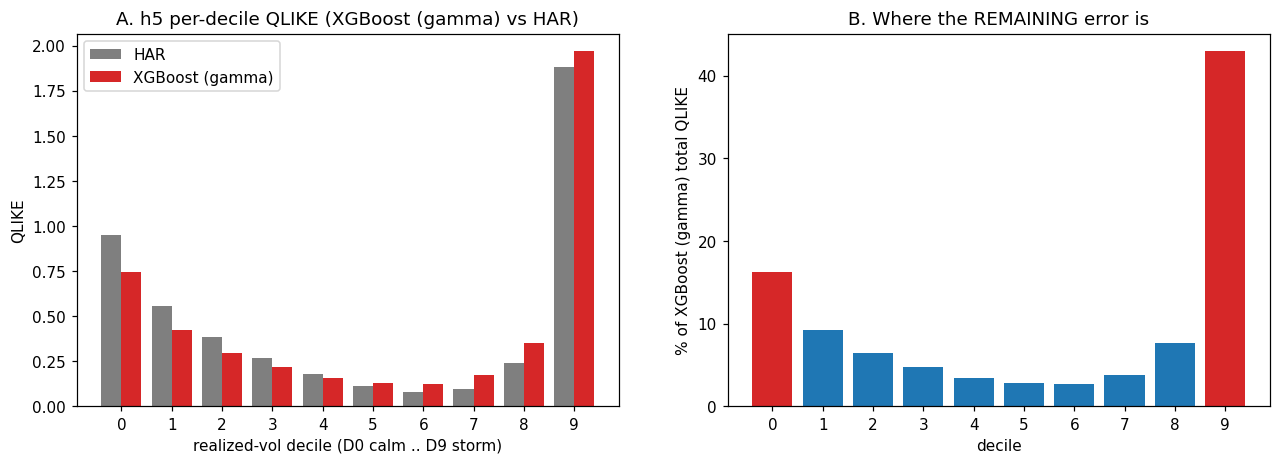
\includegraphics[width=0.85\textwidth]{fig_remaining_error_by_decile.png}
\caption{The endogenous XGBoost model beats HAR on the calm deciles, and its remaining QLIKE concentrates in
the storm decile D9, which carries 43\% of the model total.}
\label{fig:decile-error}
\end{figure}

\begin{figure}[t]
\centering
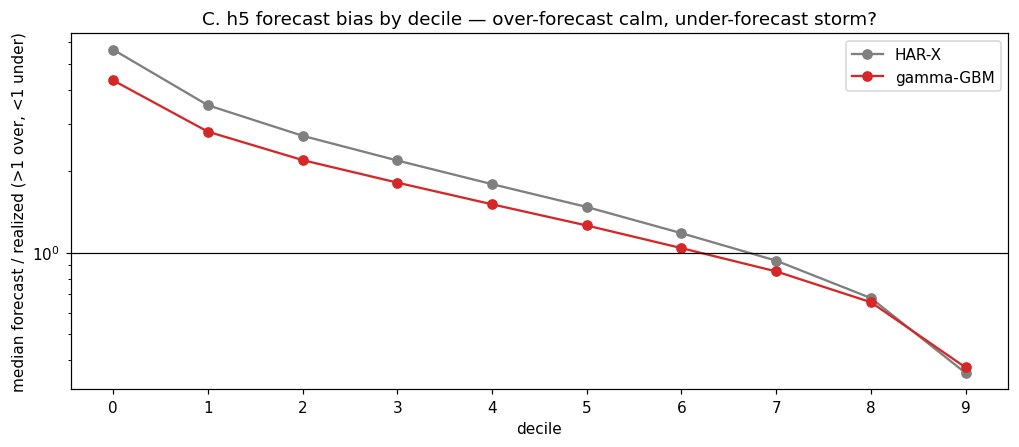
\includegraphics[width=0.85\textwidth]{fig_forecast_bias_by_decile.png}
\caption{The endogenous XGBoost model under-forecasts the storm deciles, where its median forecast-to-realized ratio drops
below one.}
\label{fig:decile-bias}
\end{figure}

\begin{figure}[t]
\centering
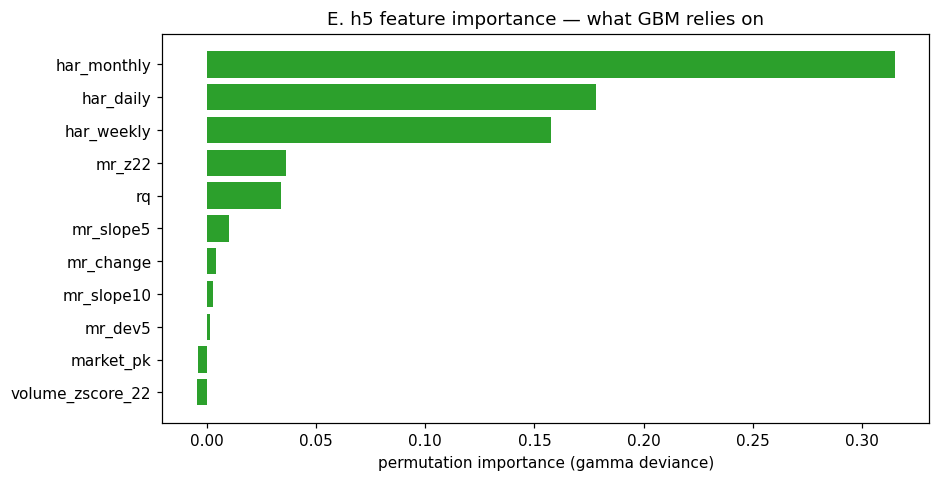
\includegraphics[width=0.85\textwidth]{fig_feature_importance.png}
\caption{Permutation importance ranks the endogenous HAR lags far above every other feature, so
endogenous is exhausted.}
\label{fig:importance}
\end{figure}

\textbf{The earnings feature is the lever.} In Table~\ref{tab:sp500}, the External earnings model
XGB+E posts the lowest QLIKE at every horizon. Against the HAR baseline the earnings model gains 14 to
16\% ($h1$ 14.3\%, $h5$ 14.9\%, $h10$ 15.0\%, $h22$ 16.1\%), which is why XGB+E carries the bolded
QLIKE in every block. % XGB+E QLIKE (leaf_graph_sp500_h*.json) vs HAR (full_compare_sp500.json)
The gain decomposes into an endogenous nonlinearity component (XGB over HAR) and an incremental earnings
component (XGB+E over XGB). On the XGBoost engine the incremental earnings component is 8.7 to 11.2\% of
QLIKE at every horizon ($h1$ 11.2\%, $h5$ 10.0\%, $h10$ 9.1\%, $h22$ 8.7\%), so the earnings block, not
the tree nonlinearity alone, drives the bulk of the S\&P~500 advantage. This earnings increment is
Diebold-Mariano-significant at every horizon ($p<0.001$).
% incremental earnings = (XGB_noearn - XGB+E)/XGB_noearn: leaf_graph_paper_sp500_noearn_h*.json metrics.XGB vs leaf_graph_sp500_h*.json metrics.XGB
% earnings-increment DM on the XGBoost engine (XGB+E vs XGB): earnings_dm_sp500.json dm_qlike h1 8.5e-61 / h5 5.0e-16 / h10 2.3e-10 / h22 2.9e-14 (all <0.001)

\textbf{Earnings do not fix the storm tail.} Decomposed by realized-volatility decile, the model's
error still concentrates in the top decile, which carries roughly ten times the calm-day QLIKE, and
its forecast-to-realized ratio there is about 0.4. The model compresses its predictions toward the
conditional mean because the storm magnitude is absent from origin-time features. The residual is
exogenous, so no origin-time feature reaches it.

\FloatBarrier
\section{Related Work}
\textbf{Neural and graph volatility forecasting.} A recent literature forecasts volatility with graph
neural networks that wire stocks through correlation or spillover edges~\cite{gnnhar2024}. We include the
published GNNHAR as a learned baseline and find, under a leakage-controlled QLIKE walk-forward, that it
does not beat a per-stock gradient-boosted tree model over endogenous features. In place of a learned
edge structure, our leaf-cooccurrence graph is derived from the forecasting model itself; it is the
boosted-tree analogue of the random-forest proximity (leaf-incidence) kernel~\cite{rhodes2023}, used
here to denoise the same-day cross-section rather than to fit a separate network. Prior Vietnamese work
builds correlation and centrality networks to predict index volatility at a monthly horizon without a
HAR or QLIKE benchmark; we extend that setting to daily per-firm QLIKE on 405 HOSE tickers.

\textbf{HAR baseline.} HAR~\cite{corsi2009} models volatility from
own history. We keep HAR as a baseline and show that a
QLIKE-loss gradient-boosted tree model~\cite{friedman2001,chen2016} with an External earnings feature
dominates them, while QLIKE~\cite{patton2011} and the Diebold-Mariano
test~\cite{dm1995,hln1997} provide the proxy-robust evaluation.

\FloatBarrier
\section{Multi-Market Replication: Vietnam HOSE}\label{sec:hose}
We replicate the study on a second, structurally different market. On 405 Ho Chi Minh Stock Exchange
(HOSE) tickers under the identical protocol, forecasting daily Parkinson variance at the same four
horizons with 390{,}577 to 399{,}040 stock-day observations per horizon, the endogenous XGBoost model
again wins, the earnings lever does not transfer, and a leaf-cooccurrence graph is a small but
significant positive lever.

\textbf{The endogenous model wins on HOSE too.} Table~\ref{tab:hose} reports all four
metrics. The endogenous XGBoost model is the DM-verified best of the non-graph models at every
horizon, while HAR trails by a wide margin. The External earnings feature does not improve it:
XGB+E is within about 0.2\% of XGB at every horizon (QLIKE 1.569 against 1.568 at $h1$ and 1.651
against 1.647 at $h5$), consistent with the flat HOSE earnings event study. The learned GNNHAR again
loses to the XGBoost model at every horizon (QLIKE worse by 4.9 to 7.1\%, DM $p<10^{-26}$).
% GNNHAR (gnnhar_hose.json) vs XGB+E (leaf_graph_hose_h{1,5}.json): (1.682-1.569)/1.569, (1.744-1.651)/1.651 Adding the
leaf-graph (XGB+E+LG) is the only change that significantly lowers QLIKE, and it carries the bolded
QLIKE at $h1$ and $h5$ (at $h10$ the leaf-graph still significantly lowers QLIKE over XGB+E, but the
earnings-inert endogenous XGB is the column minimum, as at $h22$).

\begin{table}[!ht]
\centering
\caption{Multi-market replication, HOSE (405 tickers; 390{,}577 to 399{,}040 stock-day observations per
horizon). Lower is better on every metric. MSE $\times10^{-6}$, RMSE/MAE $\times10^{-3}$; QLIKE
unscaled. GARCH is a
per-stock GARCH(1,1) benchmark; all its metrics (including the squared-error columns) are scored over
its estimable subset ($\sim$98.6\% of rows), a slightly different sample than the other models. XGB is the endogenous model, XGB+E
adds the earnings block, and XGB+E+LG adds leaf-graph smoothing. Bold marks the best value in each
metric column per horizon; the QLIKE bold additionally requires a significant date-clustered
Diebold-Mariano test ($p<0.05$).}
\label{tab:hose}
\footnotesize
\setlength{\tabcolsep}{6pt}
% [!ht] + trailing \FloatBarrier keep Table 2 near its Section 6 reference (else it floats to the last page)
\begin{tabular}{llcccc}
\toprule
$h$ & Model & MSE & RMSE & MAE & QLIKE \\
\midrule
1 & GARCH       & 0.630 & 0.794 & 0.487 & 1.656 \\ % garch_hose.json h1 GARCH (estimable subset; mse 6.299e-7, rmse 7.936e-4, mae 4.866e-4, qlike 1.6563)
1 & HAR         & 0.660 & 0.813 & 0.519 & 1.812 \\ % full_compare_hose.json h1 metrics.HAR (mse 6.6038e-7, rmse 8.1264e-4, mae 5.1928e-4, qlike 1.81169)
1 & GNNHAR      & 0.585 & 0.765 & 0.438 & 1.682 \\ % gnnhar_hose.json metrics.GNNHAR_h1 (mse 5.8472e-7, rmse 7.6467e-4, mae 4.3832e-4, qlike 1.68233)
1 & XGB         & 0.534 & 0.731 & 0.392 & 1.568 \\ % leaf_graph_paper_hose_noearn_h1.json metrics.XGB
1 & XGB+E       & 0.535 & 0.731 & 0.393 & 1.569 \\ % leaf_graph_hose_h1.json metrics.XGB
1 & XGB+E+LG    & \textbf{0.534} & \textbf{0.731} & \textbf{0.391} & \textbf{1.565} \\ % leaf_graph_hose_h1.json metrics.XGB+leafgraph (DM +0.25% p=3.6e-4, spike-robust)
\midrule
5 & GARCH       & 0.703 & 0.838 & 0.537 & 1.740 \\ % garch_hose.json h5 GARCH (estimable subset; mse 7.028e-7, rmse 8.383e-4, mae 5.370e-4, qlike 1.7401)
5 & HAR         & 0.663 & 0.814 & 0.523 & 1.822 \\ % full_compare_hose.json h5 metrics.HAR (mse 6.6264e-7, rmse 8.1403e-4, mae 5.2273e-4, qlike 1.82180)
5 & GNNHAR      & 0.616 & 0.785 & 0.469 & 1.744 \\ % gnnhar_hose.json metrics.GNNHAR_h5 (mse 6.1615e-7, rmse 7.8495e-4, mae 4.6865e-4, qlike 1.74387)
5 & XGB         & 0.578 & 0.760 & 0.425 & 1.647 \\ % leaf_graph_paper_hose_noearn_h5.json metrics.XGB
5 & XGB+E       & 0.579 & 0.761 & 0.426 & 1.651 \\ % leaf_graph_hose_h5.json metrics.XGB
5 & XGB+E+LG    & \textbf{0.578} & \textbf{0.760} & \textbf{0.424} & \textbf{1.647} \\ % leaf_graph_hose_h5.json metrics.XGB+leafgraph (DM +0.26% p=3.1e-5, spike-robust)
\midrule
10 & GARCH       & 0.734 & 0.857 & 0.565 & 1.782 \\ % garch_hose.json h10 GARCH (estimable subset; mse 7.344e-7, rmse 8.570e-4, mae 5.653e-4, qlike 1.7823)
10 & HAR         & 0.666 & 0.816 & 0.525 & 1.828 \\ % full_compare_hose.json h10 metrics.HAR (mse 6.6598e-7, rmse 8.1607e-4, mae 5.2496e-4, qlike 1.82766)
10 & GNNHAR      & 0.628 & 0.792 & 0.483 & 1.767 \\ % gnnhar_hose.json metrics.GNNHAR_h10 (mse 6.2772e-7, rmse 7.9229e-4, mae 4.8264e-4, qlike 1.76702)
10 & XGB         & 0.595 & 0.771 & \textbf{0.439} & \textbf{1.682} \\ % leaf_graph_paper_hose_noearn_h10.json metrics.XGB (n_folds=8; mse 5.9463e-7, rmse 7.711e-4, mae 4.389e-4=0.438897 min, qlike 1.6816=1.681571 min)
10 & XGB+E       & 0.595 & 0.771 & 0.441 & 1.684 \\ % leaf_graph_hose_h10.json metrics.XGB
10 & XGB+E+LG    & \textbf{0.595} & \textbf{0.771} & 0.439 & 1.682 \\ % leaf_graph_hose_h10.json metrics.XGB+leafgraph (mse 5.9462e-7/rmse 7.7111e-4 min; MAE 0.439102>XGB 0.438897 so MAE bold=XGB; leaf DM vs XGB+E +0.12% p=4.6e-3, spike-robust)
\midrule
22 & GARCH       & 0.788 & 0.888 & 0.606 & 1.837 \\ % garch_hose.json h22 GARCH (estimable subset; mse 7.879e-7, rmse 8.877e-4, mae 6.064e-4, qlike 1.8366)
22 & HAR         & 0.672 & 0.820 & 0.528 & 1.835 \\ % full_compare_hose.json h22 metrics.HAR (mse 6.7162e-7, rmse 8.1952e-4, mae 5.2816e-4, qlike 1.83547)
22 & GNNHAR      & 0.655 & 0.809 & 0.507 & 1.810 \\ % gnnhar_hose.json metrics.GNNHAR_h22 (mse 6.5453e-7, rmse 8.0903e-4, mae 5.0689e-4, qlike 1.81018)
22 & XGB         & 0.621 & 0.788 & \textbf{0.459} & \textbf{1.725} \\ % leaf_graph_paper_hose_noearn_h22.json metrics.XGB (n_folds=8; mse 6.2128e-7, rmse 7.882e-4, mae 4.591e-4, qlike 1.7251) -- endogenous is min QLIKE/MAE at h22 (earnings inert)
22 & XGB+E       & 0.622 & 0.789 & 0.461 & 1.727 \\ % leaf_graph_hose_h22.json metrics.XGB
22 & XGB+E+LG    & \textbf{0.621} & \textbf{0.788} & 0.460 & 1.726 \\ % leaf_graph_hose_h22.json metrics.XGB+leafgraph (leaf gain ns, DM p=0.34)
\bottomrule
\end{tabular}
\end{table}
\FloatBarrier

\textbf{The leaf-cooccurrence graph is a positive lever on HOSE.} Smoothing the forecasts over the
per-day leaf-cooccurrence graph lowers QLIKE relative to the unsmoothed model at the one-, five-, and
ten-day horizons: the gain is 0.25\% ($h1$, DM $p<0.001$), 0.26\% ($h5$, DM $p<0.001$), and 0.12\%
($h10$, DM $p<0.01$), and is not significant at $h22$ (0.03\%, DM $p=0.34$).
% gains + DM: leaf_graph_hose_h{1,5,10,22}.json gain_pct / dm.XGB+leafgraph_vs_XGB
The gains survive the spike-robustness screen: excluding the COVID, 2022, and April 2025 tariff windows
(57{,}466 observations), the leaf-graph still beats the unsmoothed model at $h1$, $h5$, and $h10$
(ex-spike gain 0.25\%, 0.20\%, and 0.12\%; DM $p<0.01$).
% ex-spike: leaf_graph_hose_h{1,5,10}.json spike_robustness.gain_pct_ex_spike / dm_p_ex_spike
The lever is endogenous denoising, not an earnings effect: it survives the no-earnings ablation, where
XGB+E+LG over the endogenous XGB gains 0.22\% at $h1$ (DM $p<0.001$) and 0.12\% at $h5$ (DM $p<0.001$).
% no-earn: leaf_graph_paper_hose_noearn_h{1,5}.json gain_pct / dm
The smoothing weight $\alpha$, fit per fold on validation, averages about 0.26 to 0.35 on HOSE, so the
graph is materially active there. Applying the same smoothing to the alternative HistGradientBoosting
engine did not yield a significant gain, so the effect is specific to the leaf structure exposed by the
XGBoost trees; this is why the study uses XGBoost as the forecasting engine. On the liquid S\&P~500 the
same construction is inert: the validation-fit weight collapses toward zero (mean $\alpha$ 0.00 to
0.05), and the QLIKE change is within 0.04\% and never a significant improvement, so the graph
correctly switches itself off where the cross-section is already well estimated.
% SP500 alpha + gains: leaf_graph_sp500_h{1,5,10,22}.json alpha.mean / gain_pct / dm

\textbf{Earnings does not transfer to Vietnam.} Using real crawled Vietnam announcement dates, XGB+E is
within about 0.2\% of the endogenous XGB at every horizon. A per-stock, per-day diagnostic on the HOSE
test set locates two compounding causes. First, the feature fires on only 5.6\% of test observations,
and 0.84\% before 2025, so it cannot move the pooled metric across most of the panel. Second, where it
fires the volatility response is muted: realized variance on announcement-proximate days runs about
1.1 times the baseline, against the pronounced S\&P~500 earnings spike, because Vietnam's daily price
limits cap the informational jump. The no-transfer result holds in the well-covered 2025-2026 folds,
so it does not rest on missing dates in that window.

\textbf{The HOSE result is robust to regime spikes.} The endogenous XGBoost model beats HAR at every
horizon by about 13\% on QLIKE (at $h1$, 1.569 against HAR's 1.812, a 13.4\% gain), and the advantage
persists after excluding the COVID (February to April 2020), 2022, and April 2025 tariff shock windows.
% XGB vs HAR: leaf_graph_hose_h1.json metrics.XGB vs full_compare_hose.json HAR
The endogenous advantage is a calm-market property, not an artifact of a few crisis days.

\textbf{Takeaway.} The endogenous XGBoost model wins on a second, structurally different market. The
earnings lever is specific to the S\&P~500 and does not generalize to HOSE under the available real
announcement dates, whereas the leaf-cooccurrence graph is a small but significant lever on the thin
HOSE market and self-disables on the liquid S\&P~500.

\section{Limitations}
\noindent\textbf{Earnings dates.} The S\&P~500 earnings dates are announcement dates from Yahoo Finance
(via yfinance), a single source capped at 100 events per ticker (older quarters are truncated); the
feature measures distance to the nearest such release from an archive that records realized dates, not a
point-in-time scheduling snapshot. A
date-jitter check shows the gain does not depend on exact-date timing: perturbing every S\&P~500
earnings date by a uniform random offset, the $h1$ QLIKE gain over endogenous falls from 11.1\% with
true dates to 9.0\% at plus or minus one trading day, 6.6\% at plus or minus three days, and 4.5\% at
plus or minus five days, and stays positive at every horizon. As a stronger, strictly leakage-safe
check, we recompute the gain under a point-in-time schedule in which each release date is predicted from
the firm's own past reporting cadence (the previous release plus its median inter-release gap, using only
prior releases, so no exact-date foreknowledge enters). Even under this conservative schedule the
S\&P~500 earnings gain (XGBoost engine) stays 2.8 to 3.3\% and Diebold-Mariano-significant at every
horizon ($h1$ 3.3\%, $h5$ 3.2\%, $h10$ 3.1\%, $h22$ 2.8\%; all $p<0.001$), against 8.7 to 11.2\% with the
archived dates, so the lever is not an artifact of exact-date foreknowledge; the true point-in-time gain
lies between these bounds, as confirmed release dates are typically known weeks ahead of the cadence guess.
% PIT-cadence robustness: earnings_pit_sp500.json (SP500, 8-fold x 3-seed) pit_cadence.earn_gain_pct h1 3.29 / h5 3.15 / h10 3.11 / h22 2.78 (dm_p all <1e-4); actual 11.17/9.97/9.18/8.73

\noindent\textbf{Vietnam coverage.} The HOSE earnings dates are real disclosure dates merged from two
crawlers---the State Securities Commission disclosure portal (dense only for 2025-01 through 2026-09) and
a sparse 2016-2026 vnstock news feed covering roughly 218 tickers---with no imputation and no
legal-deadline substitution. Unlike the S\&P~500, each HOSE quarter emits several distinct filings
(parent, consolidated, and combined statements across quarterly, semi-annual, and annual periods), so a
firm's disclosure cadence is far more irregular: its own-cadence date is predictable to a median of only
26 days, against 2 days on the S\&P~500. This irregular, multi-event-type schedule---not a date-accuracy
defect---makes the scheduled-earnings feature much noisier on HOSE, which is the honest reason the earnings
lever does not transfer. We therefore claim no incremental earnings value on HOSE under the available real
dates, rather than a definitive full-history null.

\noindent\textbf{Earnings decomposition.} The S\&P~500 endogenous-to-earnings decomposition (8.7 to
11.2\% incremental earnings component at every horizon) is measured on the XGBoost engine reported in the
results table. The date-jitter robustness figures below are measured on the capacity-matched
HistGradientBoosting engine.

\noindent\textbf{Leaf-graph scope.} The leaf-cooccurrence graph is a small, thin-market lever: it helps
on HOSE at the shorter horizons and self-disables on the liquid S\&P~500. Its mechanism is
cross-sectional denoising of the model's own forecasts rather than new information from outside the
stock's history, and the gains, while significant, are on the order of a few tenths of a percent.

\noindent\textbf{Scope.} The analysis is conditional on the Parkinson daily-OHLC regime and does not
speak to intraday or option-implied signals.

\section{Conclusion}
We built a per-stock volatility forecasting model on a gamma-loss gradient-boosted tree ensemble
(XGBoost) over endogenous features and asked where extra information helps. The endogenous model beats
the HAR and GARCH benchmarks and a learned graph neural network (GNNHAR) at every horizon. On the
S\&P~500, an External, forward-looking scheduled-earnings feature is the dominant lever, cutting QLIKE by
14 to 16\% over HAR at every horizon (Diebold-Mariano $p<0.001$). We replicated the study on 405 Vietnam
HOSE tickers under an identical protocol: the endogenous model again wins and the earnings lever does
not transfer, which localizes the earnings gain to the S\&P~500. On the thin HOSE market a
leaf-cooccurrence graph that denoises each day's cross-section of forecasts is a small but significant
lever at the shorter horizons, and it self-disables on the liquid S\&P~500. The practical takeaway is
that, for daily volatility, a strong endogenous model plus a market-appropriate external signal is what
matters, and the value of that signal depends on the market's information and microstructure.

\begin{thebibliography}{99}
\bibitem{corsi2009} Corsi, F.: A simple approximate long-memory model of realized volatility. J. Financial Econometrics \textbf{7}(2), 174--196 (2009)
\bibitem{parkinson1980} Parkinson, M.: The extreme value method for estimating the variance of the rate of return. J. Business \textbf{53}(1), 61--65 (1980)
\bibitem{patton2011} Patton, A.J.: Volatility forecast comparison using imperfect volatility proxies. J. Econometrics \textbf{160}(1), 246--256 (2011)
\bibitem{dm1995} Diebold, F.X., Mariano, R.S.: Comparing predictive accuracy. J. Business \& Economic Statistics \textbf{13}(3), 253--263 (1995)
\bibitem{hln1997} Harvey, D., Leybourne, S., Newbold, P.: Testing the equality of prediction mean squared errors. Int. J. Forecasting \textbf{13}(2), 281--291 (1997)
\bibitem{friedman2001} Friedman, J.H.: Greedy function approximation: a gradient boosting machine. Annals of Statistics \textbf{29}(5), 1189--1232 (2001)
\bibitem{patell1981} Patell, J.M., Wolfson, M.A.: The ex ante and ex post price effects of quarterly earnings announcements reflected in option and stock prices. J. Accounting Research \textbf{19}(2), 434--458 (1981)
\bibitem{gnnhar2024} Zhang, C., Pu, X., Cucuringu, M., Dong, X.: Graph neural networks for forecasting realized volatility with nonlinear spillover effects. Int. J. Forecasting (2024). arXiv:2308.01419
\bibitem{chen2016} Chen, T., Guestrin, C.: XGBoost: a scalable tree boosting system. In: Proceedings of the 22nd ACM SIGKDD International Conference on Knowledge Discovery and Data Mining, pp. 785--794 (2016)
\bibitem{rhodes2023} Rhodes, J.S., Cutler, A., Moon, K.R.: Geometry- and accuracy-preserving random forest proximities. IEEE Trans. Pattern Analysis and Machine Intelligence \textbf{45}(9), 10947--10959 (2023)
\end{thebibliography}

\end{document}
